\chapter{Clustering --- k-Means, GMMs, and DBSCAN}
\label{ch:lesson19}

Every prior chapter in this part assumed some \emph{target} --- a threshold, a template, a known transform. \textbf{Clustering} asks a different kind of question, with no target at all: given a pile of points (or pixels), group them into a small number of sensible categories, using only how similar they are to each other. This is \textbf{unsupervised learning}'s classical starting point --- no labels, just a distance function and an assumption about what ``a cluster'' should look like. This chapter builds three clustering algorithms from scratch, each built on a different assumption about cluster shape, and shows concretely where each one wins and fails: \textbf{k-means} (round, similarly-sized clusters), \textbf{Gaussian mixture models} (elliptical clusters, soft assignment), and \textbf{DBSCAN} (arbitrary shape, defined by density rather than a center).

\section{k-means on real color data}

Chapter~\ref{ch:lesson18} built a perceptually meaningful color distance (L*a*b* Euclidean distance). Clustering is the natural next step: given a pile of pixel colors and no labels at all, group them into regions automatically.

K-means, also known as Lloyd's algorithm, is here unchanged from its textbook form: pick $k$ random points as initial centers, assign every point to its nearest center, recompute each center as the mean of its assigned points, repeat until nothing moves.

\begin{figure}[h]
\centering
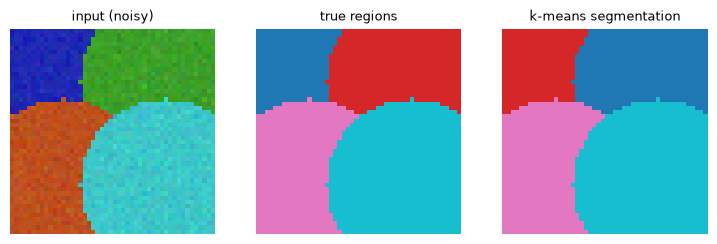
\includegraphics[width=0.9\textwidth]{figures/lesson19_fig01.png}
\caption{A synthetic noisy 4-region color image, the true regions, and the k-means segmentation on L*a*b* pixel colors --- purity $1.000$ against the true regions.}
\label{fig:l19-1}
\end{figure}

With compact, roughly equal-sized, roughly round clusters in L*a*b* space (exactly what this synthetic image has), k-means recovers the true regions almost perfectly, as Figure~\ref{fig:l19-1} shows. Two real caveats worth flagging even in this success case: $k$ (the number of clusters) has to be chosen in advance --- nothing in the algorithm discovers it --- and different random initializations can converge to different, sometimes noticeably worse, local optima; \textbf{k-means++} (\citelink{arthur2007}{Arthur \& Vassilvitskii, 2007}) fixes this by seeding centers to be spread apart rather than purely at random.

\section{Where k-means breaks: non-convex clusters}

K-means' update rule --- assign to the nearest \emph{center} --- can only carve space into convex regions. A dataset that isn't convex at all: two concentric rings. No placement of two centers can separate them correctly, no matter how many times the algorithm iterates. K-means lands right at chance ($54.0\%$, vs.\ $50\%$ for random guessing on this 2-class problem) --- it splits the two rings radially, half of each ring going to each cluster, because that's the only kind of boundary (a straight line, equidistant between two centers) the algorithm is capable of drawing, as Figure~\ref{fig:l19-2} shows.

\begin{figure}[h]
\centering
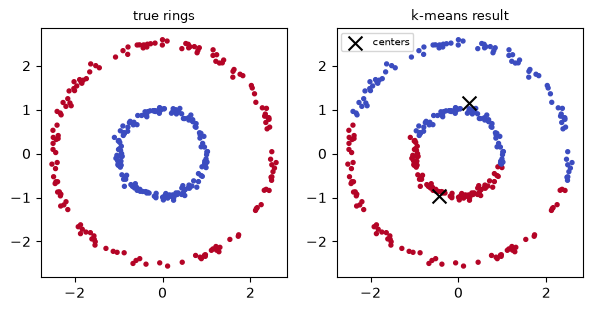
\includegraphics[width=0.7\textwidth]{figures/lesson19_fig02.png}
\caption{True concentric rings vs.\ the k-means result (centers marked with $\times$). The clusters aren't ambiguous to a human eye at all; the \emph{algorithm's assumption} (round, center-based clusters) is simply the wrong tool for this shape.}
\label{fig:l19-2}
\end{figure}

\section{Gaussian mixture models: soft, elliptical clusters}

A \textbf{Gaussian mixture model (GMM)} generalizes k-means two ways: each cluster gets its own full covariance (so clusters can be elongated ellipses, not just circles), and assignment is \emph{soft} --- every point gets a probability of belonging to each cluster, not a hard label. Fit by \textbf{expectation-maximization (EM)} (\citelink{dempster1977}{Dempster, Laird, \& Rubin, 1977}): the E-step computes each point's responsibility (probability) under the current Gaussians; the M-step re-fits each Gaussian's mean, covariance, and weight to its responsibility-weighted points.

On the concentric rings, GMM does no better than k-means: $55.7\%$ accuracy, also near chance. That's an important, easy-to-miss point: GMM fixes k-means' \emph{round-only} assumption, but it's still a \textbf{unimodal-per-cluster} model --- each cluster is described by one Gaussian bump. A ring isn't elliptical any more than it's circular; no single Gaussian, of any shape, fits an annulus well. GMM and k-means fail this dataset for the same underlying reason.

\section{DBSCAN: clusters defined by density, not shape}

\textbf{DBSCAN} (density-based spatial clustering, \citelink{ester1996}{Ester et al., 1996}) never fits a parametric shape at all. A point is a \textbf{core point} if at least \code{min\_samples} other points lie within distance \code{eps} of it. Clusters are formed by chaining together core points that are within \code{eps} of each other (and their neighbors), so a cluster can be any shape --- including a ring --- as long as it's a \emph{connected, sufficiently dense} region of space. Points that end up in no core point's neighborhood are labeled \textbf{noise}, not forced into the nearest cluster.

On the same rings: DBSCAN finds exactly 2 clusters, 0 noise points, and $100.0\%$ accuracy (Figure~\ref{fig:l19-3}).

\begin{figure}[h]
\centering
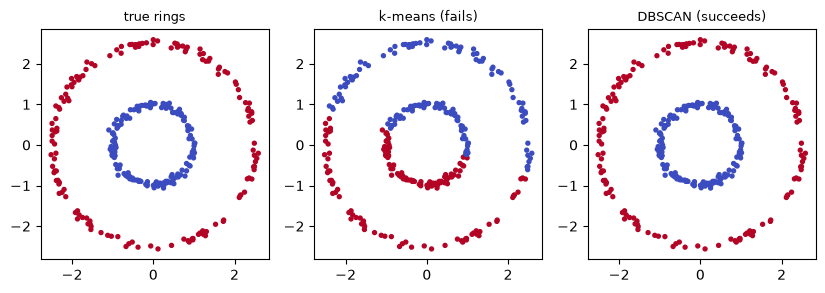
\includegraphics[width=0.95\textwidth]{figures/lesson19_fig03.png}
\caption{True rings, the k-means result (fails), and the DBSCAN result (succeeds). DBSCAN never assumed a center or a shape, only that points \emph{within} a ring are densely connected to their neighbors, while the gap between rings is not.}
\label{fig:l19-3}
\end{figure}

This comes at a real cost: \code{eps} and \code{min\_samples} have to be chosen by hand (a poor choice fragments each ring into dozens of tiny arcs), and DBSCAN struggles when different true clusters have very different densities, since one global \code{eps} can't be simultaneously right for a sparse cluster and a dense one.

\section{Noise robustness: a real advantage of ``no forced assignment''}

Add clutter --- points scattered uniformly across the whole region, belonging to neither ring --- and compare how each algorithm handles them. k-means and GMM have no concept of ``doesn't belong to any cluster'': every point gets assigned somewhere, dragging cluster centers toward the clutter. DBSCAN can simply call clutter what it is: out of 60 clutter points added, k-means correctly flags $0$ as anything other than ``definitely part of a ring'' (it has no vocabulary for that at all), while DBSCAN correctly isolates $8$ of them as noise. The rest happen to land within \code{eps} of a real ring point (or of each other, forming a small cluster of their own) --- a fair outcome, not a bug, since density-based clustering only calls a point noise if it's genuinely isolated. The qualitative point stands regardless of the exact count: DBSCAN has a real, usable category for ``this doesn't fit anywhere,'' whereas k-means structurally cannot.

\section{Where this goes next}

This is the end of Part 1. Many of the algorithms encountered so far operate directly on \textbf{raw or hand-picked features} --- pixel color, $(x,y)$ coordinates, texture --- and rely on human-chosen distance functions, such as those used here. Later chapters revisit many of these problems using deep learning to automatically discover the features and the rules for combining them: Chapter 43's instance segmentation uses a similar clustering idea, and Chapter 48's autoencoder learns the feature space itself, purely from reconstruction error, before any grouping is asked for at all. Where this chapter's methods assume a shape and fit it, the deep-learning methods later in this course learn a representation and let structure emerge from it.

\subsection*{Exercises}
\begin{enumerate}
  \item Rerun the color-segmentation k-means with $k=3$ and $k=6$ instead of the true $4$. Since nothing in the algorithm can ``know'' the right number of clusters, how does the segmentation degrade in each direction, and can you tell purely from the output which $k$ is likely wrong?
  \item The GMM above was evaluated only on the ring dataset, where it fails for the same reason k-means does. Construct a two-cluster dataset where the clusters are genuinely elliptical (e.g.\ using a multivariate normal with a non-diagonal covariance) and compare GMM against k-means there. Does GMM's extra flexibility (fitting the shape, not just the center) show a real accuracy advantage this time?
  \item In the noisy-clutter DBSCAN demo, shrink \code{eps} from $0.6$ to $0.3$. Does DBSCAN start mislabeling real ring points as noise, real clutter points as belonging to a ring, or both --- and does that match the earlier warning about \code{eps} being a hand-tuned, dataset-specific choice rather than something the algorithm discovers?
\end{enumerate}

\vfill
\fullcode{lesson19}{lesson19_clustering}
